\subsection{The Shapley values of the five switches}
\label{sec:ablation-shapley}

Table~\ref{tab:shapley} gives the exact Shapley value of each switch for the two measures in the three variants whose net UF position is 30 percent of level 1 capital, and Figure~\ref{fig:shapley} draws them. For the income measure the picture is that of the theory. The charge has the value $\mainShapNiiChargeLng\pm\mainShapNiiChargeLngCi$ million pesos in each of the three variants, the constant $\kappa|\PNUR|$ of Proposition~\ref{prop:shapley} with no interval because it does not vary across books. The own sizes switch has the value $\mainShapNiiSizesLng\pm\mainShapNiiSizesLngCi$, the dummy of the same proposition. The pair rule has $\mainShapNiiPairLng\pm\mainShapNiiPairLngCi$, $\mainShapNiiPairSht\pm\mainShapNiiPairShtCi$ and $\mainShapNiiPairOff\pm\mainShapNiiPairOffCi$, a little more than half of the charge, and the own curve and the own floor are small, $\mainShapNiiCurveLng\pm\mainShapNiiCurveLngCi$ and $\mainShapNiiFloorLng\pm\mainShapNiiFloorLngCi$ in the long UF variant, because they act only when the floor of zero binds on the low short rates of the UF curve. The income gap between the two treatments is therefore carried by the aggregation and the charge, in the proportion of about one to two.

\begin{table}[htbp]
\centering
\footnotesize
\setlength{\tabcolsep}{3.5pt}
\caption{Exact Shapley value of each of the five switches that turn the single-currency treatment of the UF leg into the Annex 1 treatment, for the three variants with a net UF position of 30 percent of level 1 capital, as the mean and the 95 percent half-width over 30 synthetic books; each panel's last row is the Annex 1 measure minus the single-currency measure, which the five values add up to.}
\label{tab:shapley}
\begin{tabular}{lrrr}
\toprule
\multicolumn{4}{l}{\textbf{Panel A. Delta EVE, CLP million}} \\
\midrule
Switch turned on & Long UF & Short UF & Offset on/off \\
\midrule
Own curve & 32{,}767$\pm$956 & 18{,}927$\pm$1{,}029 & 32{,}724$\pm$976 \\
Own shock sizes & $-$28{,}757$\pm$568 & $-$8{,}379$\pm$597 & $-$28{,}671$\pm$628 \\
Own floor & 0$\pm$0 & 0$\pm$0 & 0$\pm$0 \\
Pair rule with offset & 866$\pm$367 & 0$\pm$0 & 13{,}346$\pm$468 \\
Indexation charge & 0$\pm$0 & 0$\pm$0 & 0$\pm$0 \\
Sum: Annex 1 minus single currency & 4{,}875 & 10{,}548 & 17{,}399 \\
\midrule
\multicolumn{4}{l}{\textbf{Panel B. Delta NII, CLP million}} \\
\midrule
Switch turned on & Long UF & Short UF & Offset on/off \\
\midrule
Own curve & 283$\pm$139 & 421$\pm$163 & 475$\pm$172 \\
Own shock sizes & 0$\pm$0 & 0$\pm$0 & 0$\pm$0 \\
Own floor & $-$172$\pm$101 & $-$257$\pm$122 & $-$295$\pm$130 \\
Pair rule with offset & 3{,}202$\pm$99 & 3{,}283$\pm$97 & 3{,}315$\pm$96 \\
Indexation charge & 6{,}182$\pm$0 & 6{,}182$\pm$0 & 6{,}182$\pm$0 \\
Sum: Annex 1 minus single currency & 9{,}495 & 9{,}630 & 9{,}677 \\
\bottomrule
\end{tabular}
\end{table}


For the value measure the picture is different, and it is the result that refutes H2. The own curve has the value $\mainShapEveCurveLng\pm\mainShapEveCurveLngCi$, $\mainShapEveCurveSht\pm\mainShapEveCurveShtCi$ and $\mainShapEveCurveOff\pm\mainShapEveCurveOffCi$ million pesos in the three variants, and the own sizes $\mainShapEveSizesLng\pm\mainShapEveSizesLngCi$, $\mainShapEveSizesSht\pm\mainShapEveSizesShtCi$ and $\mainShapEveSizesOff\pm\mainShapEveSizesOffCi$, with the opposite sign. The two nearly cancel in the long UF and the offset variants, so that the difference of the two measures, \repAnnexEveLng{} against \repSingleEveLng{} million pesos at the committed seed in the long UF variant, is a small remainder of two large terms. The pair rule has $\mainShapEvePairLng\pm\mainShapEvePairLngCi$, $\mainShapEvePairSht\pm\mainShapEvePairShtCi$ and $\mainShapEvePairOff\pm\mainShapEvePairOffCi$: it matters for the value measure only in the offset variant, whose peso bonds are twice as long and whose legs move in opposite directions at several scenarios, and not where the argmax scenario is the parallel-up shock at which both legs lose. The floor and the charge are zero, the floor because no floor binds in a value scenario that attains the maximum, the charge by construction.

\begin{figure}[htbp]
\centering
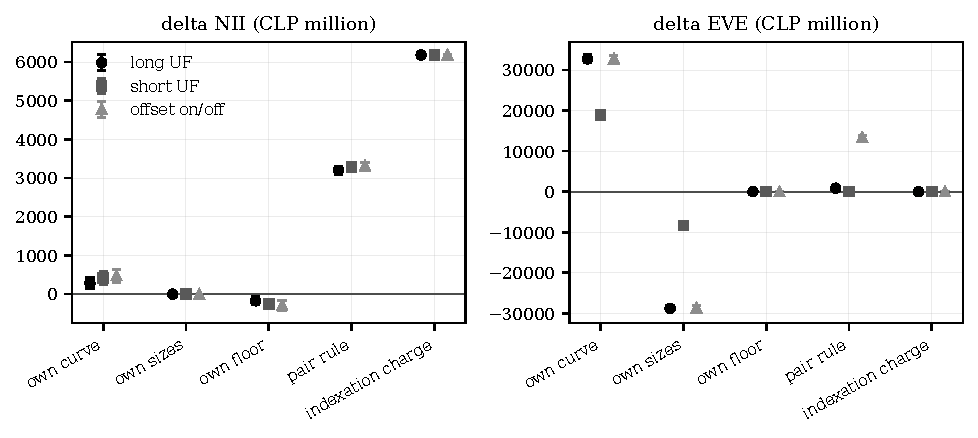
\includegraphics[width=\textwidth]{shapley-values}
\caption{Exact Shapley value of each of the five switches for the delta NII (left) and the delta EVE (right) in the three variants with a 30 percent net UF position, as means over 30 synthetic books with 95 percent intervals.}
\label{fig:shapley}
\end{figure}

\subsection{One at a time, and the interaction between the switches}
\label{sec:ablation-oat}

Table~\ref{tab:ablation} gives, for the long UF variant, the change of each measure when a switch is turned off in the Annex 1 treatment, the change when it alone is turned on in the single-currency treatment, and the Shapley value. For the value measure, turning the own curve on alone adds $\mainAoiEveCurveLng$ million pesos, turning it off in Annex 1 removes $\mainLooEveCurveLng$ and the Shapley value is $\mainShapEveCurveLng$: the three differ by about 20 percent, which is the interaction of the curve with the sizes, since the first-order weight $w_k$ of Equation~\eqref{eq:weight} depends on both. The same holds for the sizes, $\mainAoiEveSizesLng$, $\mainLooEveSizesLng$ and $\mainShapEveSizesLng$. For the income measure the three quantities coincide for the charge ($\mainAoiNiiChargeLng$, $\mainLooNiiChargeLng$, $\mainShapNiiChargeLng$) and for the pair rule to within the width of the interval ($\mainAoiNiiPairLng$, $\mainLooNiiPairLng$, $\mainShapNiiPairLng$): the additive switches do not interact, which is what makes the attribution of the income gap unambiguous. The own curve has a first-order effect of $\mainAoiNiiCurveLng$ when it acts alone and none when it is turned off in Annex 1, an interaction with the floor: with the peso floor of zero the fall of 300 basis points takes the low UF rates below zero and the floor binds, which changes the income measure, and with the floor of minus two percent it does not bind, so the curve then changes nothing (Proposition~\ref{prop:floor}). No other switch changes sign across the three quantities.

\begin{table}[htbp]
\centering
\footnotesize
\setlength{\tabcolsep}{3.5pt}
\caption{One-at-a-time ablation on the long UF variant, as the mean and the 95 percent half-width over 30 books: the change of the measure when a switch is turned off in Annex 1 (the first column is the measure without the switch minus the Annex 1 measure) and when it alone is turned on in the single-currency treatment, beside the Shapley value that averages the change over every order of the five switches.}
\label{tab:ablation}
\begin{tabular}{lrrr}
\toprule
\multicolumn{4}{l}{\textbf{Panel A. Delta EVE, long UF variant, CLP million}} \\
\midrule
Switch & Annex 1 without it & Single currency with it & Shapley value \\
\midrule
Own curve & $-$27{,}228$\pm$800 & 38{,}306$\pm$1{,}112 & 32{,}767$\pm$956 \\
Own shock sizes & 34{,}296$\pm$704 & $-$23{,}218$\pm$446 & $-$28{,}757$\pm$568 \\
Own floor & 0$\pm$0 & 0$\pm$0 & 0$\pm$0 \\
Pair rule with offset & $-$866$\pm$367 & 866$\pm$367 & 866$\pm$367 \\
Indexation charge & 0$\pm$0 & 0$\pm$0 & 0$\pm$0 \\
\midrule
\multicolumn{4}{l}{\textbf{Panel B. Delta NII, long UF variant, CLP million}} \\
\midrule
Switch & Annex 1 without it & Single currency with it & Shapley value \\
\midrule
Own curve & 0$\pm$0 & 787$\pm$357 & 283$\pm$139 \\
Own shock sizes & 0$\pm$0 & 0$\pm$0 & 0$\pm$0 \\
Own floor & 122$\pm$134 & 0$\pm$0 & $-$172$\pm$101 \\
Pair rule with offset & $-$3{,}313$\pm$125 & 3{,}313$\pm$125 & 3{,}202$\pm$99 \\
Indexation charge & $-$6{,}182$\pm$0 & 6{,}182$\pm$0 & 6{,}182$\pm$0 \\
\bottomrule
\end{tabular}
\end{table}


Two conclusions follow for the use of the measure. A reader who wants to know what the separate treatment adds to the income measure can read it from two numbers, the charge and the offset, and the sum is stable across books. A reader who wants the same for the value measure cannot read it from the sum: the gap between the two treatments is small because a real curve that raises the sensitivity of the UF flows and a smaller table of sizes that lowers it nearly offset each other, and a change in either input of the supervisor's text, a recalibrated size table for example, would move the gap by tens of thousands of millions of pesos without any change in the treatment of the UF as a currency.
